\documentclass{article}
\usepackage{graphicx}
\graphicspath{{images/}}
\usepackage{hyperref}
\title{TP 4A - Génie Logiciel
Programme Java intégrant modélisation UML, versionning (git)
et tests unitaires (Junit)
}
\author{Mathis Vaugeois - Tanguy Moriceau - Faustine Guillou}
\date{January 2023}

\begin{document}

\maketitle
\tableofcontents

\newpage
\section{Introduction}
\subsection{Context}

\subsection{Git}

Pour travailler en groupe, Nous avons décidé d'appliquer ce que nous avions appris en cours : Git. Nous avons mis proprement à jour nos comptes GitHub. Mathis a créé

\newpage
\section{Cahier des charges}
\subsection{Exercice 1}

\begin{figure}
    \centering
    \includegraphics[width=0.75\textwidth]{diagrammeClasse}
    \caption{Diagramme de Classe}
    \label{fig:mesh1}
\end{figure}

%\begin{figure}
    %\centering
   % \includegraphics[width=0.75\textwidth]{diagrammeSeq}
    %\caption{Diagramme de Séquence.}
    %\label{fig:mesh2}
%\end{figure}

%\begin{figure}
    %\centering
   % \includegraphics[width=0.75\textwidth]{diagrammeObj}
    %\caption{Diagramme d'Objet.}
    %\label{fig:mesh3}
%\end{figure}

1.
Voici notre diagramme UML \ref{fig:mesh1} que vous pouvez voir sur la page \pageref{fig:mesh1}.
\newline
2. Voici notre diagramme de séquence % \ref{fig:mesh2}
 que vous pouvez voir sur la page% \pageref{fig:mesh2}.
\newline
3. Nous pourrions aussi proposer un diagramme d'objet. Nous avons décidé le réaliser, le voici:
% \ref{fig:mesh3}
.Vous pouvez aussi le voir sur la page% \pageref{fig:mesh3}.


\newpage
\section{Code de départ}

\newpage
\section{Développement}
\subsection{Exercice 3 - Premiers développements}
1.

2.

3.
Les tests inutiles ont été retirés. Les tests utiles ont été déplacés dans un test Junit "TestsDossierBancaire". Des tests supplémentaires
pour tester les autres fonctionnalités de la classe DossierBancaire on été ajoutés. Le test Junit a été renommé "TestsSuite".

4.

5.
Une classe Compte a été créée. Celle-ci contient un solde (privé), ainsi qu'un constructeur et deux méthodes permettant de récupérer
le montant de ce solde, ainsi que de déposer de l'argent sur le compte.

Un attribut de type Compte a été ajouté au dossier bancaire (compteCourant), permettant d'accéder aux comptes. Le dossier bancaire
contient un constructeur (qui initialise un compteCourant), une méthode permettant de récupérer le solde du dossier bancaire, une méthode permettant de déposer de l'argent (appel de la fonction du compteCourant), une méthode permettant d'accéder au compteCourant (et d'appeller ses méthodes). Des tests ont été mis en place avec Junit.

6.
Un attribut de type Compte a été ajouté au dossier bancaire (compteEpargne), permettant d'accéder aux comptes. Le dossier bancaire
contient aussi désormais une fonction de rémunération à taux fixe, qui dépose de l'argent sur le compteEpargne, ainsi qu'une méthode permettant d'accéder au compteEpargne (et d'appeller ses méthodes). La fonction de dépot a été modifiée afin de ventiler la somme d'argent déposée. Des tests ont été mis en place avec Junit.

7, 8 et 9.
Faisables avec GitDesktop.

\subsection{Exercice 4 - Fusion}

1.
Légères modifications de la classe DossierBancaire (noms et commentaires)

2.
Faisable avec GitDekstop. Amélioration de la structure du code précédemment réalisée (lors de l'initialisation du projet). Documentation enrichie.

3.
Documentation enrichie (commentaires).

4.
Faisable avec GitDesktop. 

5.
Tests unitaires OK et GUI OK.

\subsection{Exercice 5 - Tests}

1.
Une fonction de retrait a été ajoutée à la classe DossierBancaire et permet de retirer de l'argent du compteCourant, avec vérification du 
solde préalablement à l'opération.

2.
Tests Junit mis en place pour tester le bon fonctionnement de l'implémentation.

3.
Interface GUI modifiée pour permettre le retrait depuis l'interface graphique.

4.
Faisable avec GitDesktop.

\newpage
\section*{Référence}




\url{https://github.com/mathisvaugeois/TPBank-GenieLogiciel}

\end{document}